\section{集束优化}

目前绝大多数的SLAM算法通过集束优化\citep{triggs1999bundle}(Bundle Adjustment,BA)方法来对状态进行估计在传统的视觉SfM算法中,集束优化是指通过联合优化所有的视觉观测误差来同时求解最优的相机位姿状态和路标点状态的方法。而对于使用了更多传感器的SLAM系统,除了路标点和位姿状态,集束优化算法还需要实时地、持续对系统的其他状态比作出估计。对于视觉惯性SLAM,集束优化通常会通过联合优化所有的视觉观测和惯性观测来同时求解相机或IMU的位姿、速度以及IMU的bias状态。

\subsection{基于图优化的状态估计}

图优化方法是分析并求解SLAM后端状态估计问题的常用工具。最早在机器人领域,为了解决多段激光传感器数据额融合时的全局一致性问题,\citep{lu1997globally,lu1997robot}提出了基于位姿图的优化方法。\citeauthor{thrun2006graph}在此基础上进一步提出了GraphSLAM\citep{thrun2006graph},使用由位姿状态和路标点状态以及它们之间的约束构成的因子图来描述集束优化问题。因子图可以很直观地描述集束优化问题中状态和约束之间的关联,有助于分析集束优化问题的各种性质。经过长时间的发展,图优化方法已经成为SLAM领域的经典方法。

\begin{figure}[htbp]
    \centering
    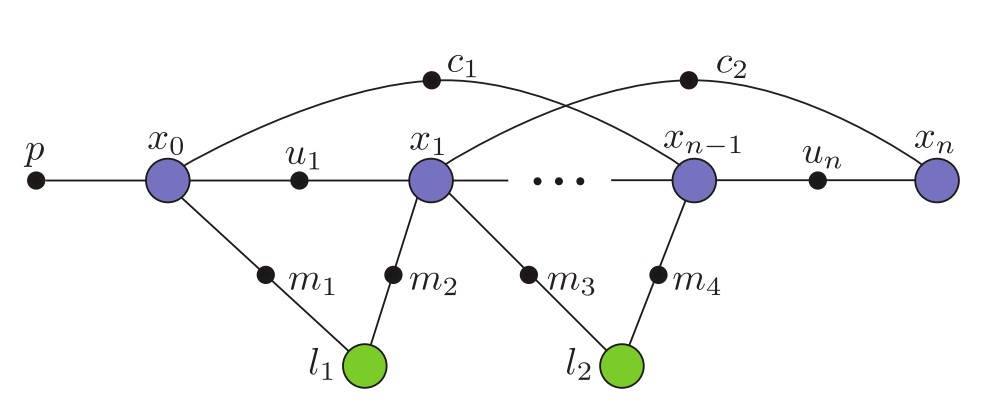
\includegraphics[width=.6\textwidth]{figs/factor_graph.png}
    \caption{因子图示例\citep{kaess2012isam2}:紫色节点代表位姿状态,绿色节点代表路标点状态,黑色节点代表状态之间的约束因子。}
    \label{fig:factor_graph}
\end{figure}

图\ref{fig:factor_graph}展示了一类常见的因子图结构。按照图示的例子,一个SLAM问题中可能存在的约束有状态变量的先验约束$p$,相邻状态之间的相对位姿约束$u_1 \dots u_n$,非相邻状态之间的回路闭合约束$c_1,c_2$以及视觉观测约束$m_1 \dots m_4$等。而求解完整集束优化的过程就相当于最大化整个因子图中的所有约束的集合$\mathcal{Z}$关于所有状态集合$\mathcal{X}$的联合条件概率:
\begin{equation}
    P(\mathcal{Z}|\mathcal{X}) = \prod_{f_i\in\mathcal{Z}} P(f_i(\mathcal{X}_i))
\end{equation}

其中$\mathcal{X}_i$代表所有与约束节点$f_i$相邻的状态节点。通常会假设这是一个高度非线性系统,并且所有的约束$f_i$的噪声服从高斯分布$f_i\sim\mathcal{N}(\mu_i, \sigma_i^2)$。这样的的概率最大化问题通常被转化为非线性最小二乘(Non-linear Least Squares,NLS)问题来求解:
\begin{equation}
\begin{aligned}
    \mathcal{X}^\ast &= \mathop{\arg\max}_{\mathcal{X}}
                        \prod_{f_i\in\mathcal{Z}} P(f_i(\mathcal{X}_i)) \\
                     &= \mathop{\arg\min}_{\mathcal{X}}
                        \sum_{f_i\in\mathcal{Z}} \frac{1}{2}
                        \lVert f_i(\mathcal{X}_i)) \rVert_{\sigma_i^2}^2
\end{aligned}
\end{equation}

\subsection{非线性最小二乘问题}

非线性最小二乘问题难以被直接求解,标准的做法是将其转化为一系列的线性最小二乘(Linear Least Squares,LLS)子问题,通过迭代求解这些子问题,来逼近原非线性最小二乘问题的局部最优解。如下给出了而一个典型的线性最小二乘问题的形式:
\begin{equation}
\begin{aligned}
    \bm{x}^\ast &= \mathop{\min}_{\bm{x}} F(\bm{x}) \\
                &= \mathop{\min}_{\bm{x}}
                   \frac{1}{2} \Vert \mathrm{A}\bm{x} + \bm{b} \Vert^2
\end{aligned}
\end{equation}

其中变量$\bm{x}$为$n$维向量,$F(\cdot)$为关于变量$\bm{x}$的标量线性函数,即能量函数。在局部最优解附近,最小化能量函数$F(\cdot)$等同于求解其梯度函数$\bm{g}(\cdot)$的零点(对于线性的函数则为唯一的零点),即:
\begin{equation}
    \bm{g} \doteq \nabla F = \begin{bmatrix}
        \frac{\partial F}{\partial x_1} &
        \frac{\partial F}{\partial x_2} &
        \cdots &
        \frac{\partial F}{\partial x_n}
    \end{bmatrix}^\top = \bm{0}
\end{equation}

Apply Newton's method, denote the first-order derivative of $\bm{g}$ as the Hessian of $\mathbf{f}(\cdot)$

\begin{equation}
    \mathrm{H} \doteq \begin{bmatrix}
        \frac{\partial^2 F}{\partial x_1^2} &
        \frac{\partial^2 F}{\partial x_1 \partial x_2} &
        \cdots & \cdots &
        \frac{\partial^2 F}{\partial x_1 \partial x_n} \\
        %
        \frac{\partial^2 F}{\partial x_2 \partial x_1} &
        \frac{\partial^2 F}{\partial x_2^2} &
        & &
        \frac{\partial^2 F}{\partial x_2 \partial x_n} \\
        %
        \vdots & & \ddots & & \vdots \\
        \vdots & & & \ddots & \vdots \\
        %
        \frac{\partial^2 F}{\partial x_n \partial x_1} &
        \frac{\partial^2 F}{\partial x_n \partial x_2} &
        \cdots & \cdots &
        \frac{\partial^2 F}{\partial x_n^2}
    \end{bmatrix}
\end{equation}

Given that $\mathrm{H}$ is rank-sufficient, due to the linearity of the gradient, it is guaranteed that we can achieve the solution by only one step starting with an arbitrary $\bm{x}$ (we choose $\bm{0}$ here) and solving the linear system

\begin{equation}
    \mathrm{H} \bm{x} = -\bm{g} \quad
    \Rightarrow \bm{x} = -\mathrm{H}^{-1} \bm{g}
\end{equation}

\subsection{高斯-牛顿法}\label{sec:gn}

For NLLS, as mentioned before, it is too expensive to compute the exact Hessian of $F(\cdot)$. We next introduce the Gauss-Newton (GN) method for solving NLLS. The main difference is that in Quasi-Newton method, one make assumption that Hessian is symmetric and use a guessed $\mathrm{B}$ to approximately replace the Hessian, while in GN method, we make the assumption that the next iteration step approximately subjects to the Gaussian distribution, thus the Hessian is naturally symmetric and positive semidefinite.

We start with the basic NLLS problem

\begin{equation}\label{eq:nlls}
\begin{aligned}
    \bm{x}^\star &= \mathop{\arg\min}_{\bm{x}} F(\bm{x}) \\
                 &= \mathop{\arg\min}_{\bm{x}}
                    \frac{1}{2} \Vert \mathbf{f}(\bm{x}) \Vert^2
\end{aligned}
\end{equation}

Using Taylor expansion and negelecting higher-order terms at every $x$

\begin{equation}
    \mathbf{f}(\bm{x}+\bm{\delta}) \simeq \mathbf{f}(\bm{x}) + \mathrm{J}\bm{\delta}
\end{equation}

results in the linearized LLS subproblem

\begin{equation}
\begin{aligned}
    \bm{\delta}_{gn} &=
        \mathop{\min}_{\bm{\delta}}
        \frac{1}{2} \Vert \mathbf{f}(\bm{x}) + \mathrm{J}\bm{\delta} \Vert^2 \\ &=
        %
        \mathop{\min}_{\bm{\delta}}
        \left( \mathbf{f}(\bm{x}) + \mathrm{J}\bm{\delta} \right)^\top
        \left( \mathbf{f}(\bm{x}) + \mathrm{J}\bm{\delta} \right) \\ &=
        %
        \mathop{\min}_{\bm{\delta}}
        \left(
            \bm{\delta}^\top \mathrm{J}^\top \mathrm{J} \bm{\delta} +
            \mathbf{f}^\top(\bm{x}) \mathrm{J} \bm{\delta} +
            \mathrm{J}^\top \mathbf{f}(\bm{x}) \bm{\delta} +
            \mathbf{f}^\top(\bm{x}) \mathbf{f}(\bm{x})
        \right)
\end{aligned}
\end{equation}

Acquiring the step $\bm{\delta}_{gn}$ is equivalent to finding the zero of the gradient of the above linearized cost function, i.e., solving the following \textbf{normal equation}

\begin{equation}
\begin{gathered}
    \mathrm{H} \bm{\delta} = -\bm{g} \\
    \mathrm{H} = \mathrm{J}^\top \mathrm{J}, \quad
    \bm{g} = \mathrm{J}^\top \mathbf{f}(\bm{x})
\end{gathered}
\end{equation}

where $\mathrm{H}$ and $\bm{g}$, we can say, are the approximated Hessian and gradient of the origin NLLS problem at linearization point $\bm{x}$.

\subsection{信赖域方法}

It has been shown that even for well-constrained nonlinear least squares problems, trust region strategies provide better performance than the Gauss-Newton method, not only in the numerical accuracy but also the rate of convergence, as they will automatically adjust the trust region radius at every iteration according to the gain ratio.

\subsection{鲁棒估计}
